\chapter{Overview of the hardware}

\section{Introduction}
The magnetometer is designed for low-power operation, simple
installation and ease of construction. The entire design is open
source, allowing anyone with reasonable soldering ability to construct
one.

The magnetometer has two major parts, the base unit and the sensor
unit (\figurename~\ref{fig:system-overview}). The sensor unit is located
outdoors, away from buildings, cars and other sources of human
disturbance. It is battery powered and communicates with the base unit
by a radio link (\MHz{433} or \MHz{868}), enabling the sensor to be
installed without any wiring to the base unit. The base unit is placed
indoors and should be positioned such that there are the minimum
number of walls between it and the sensor unit.

\begin{figure}
  \centering
  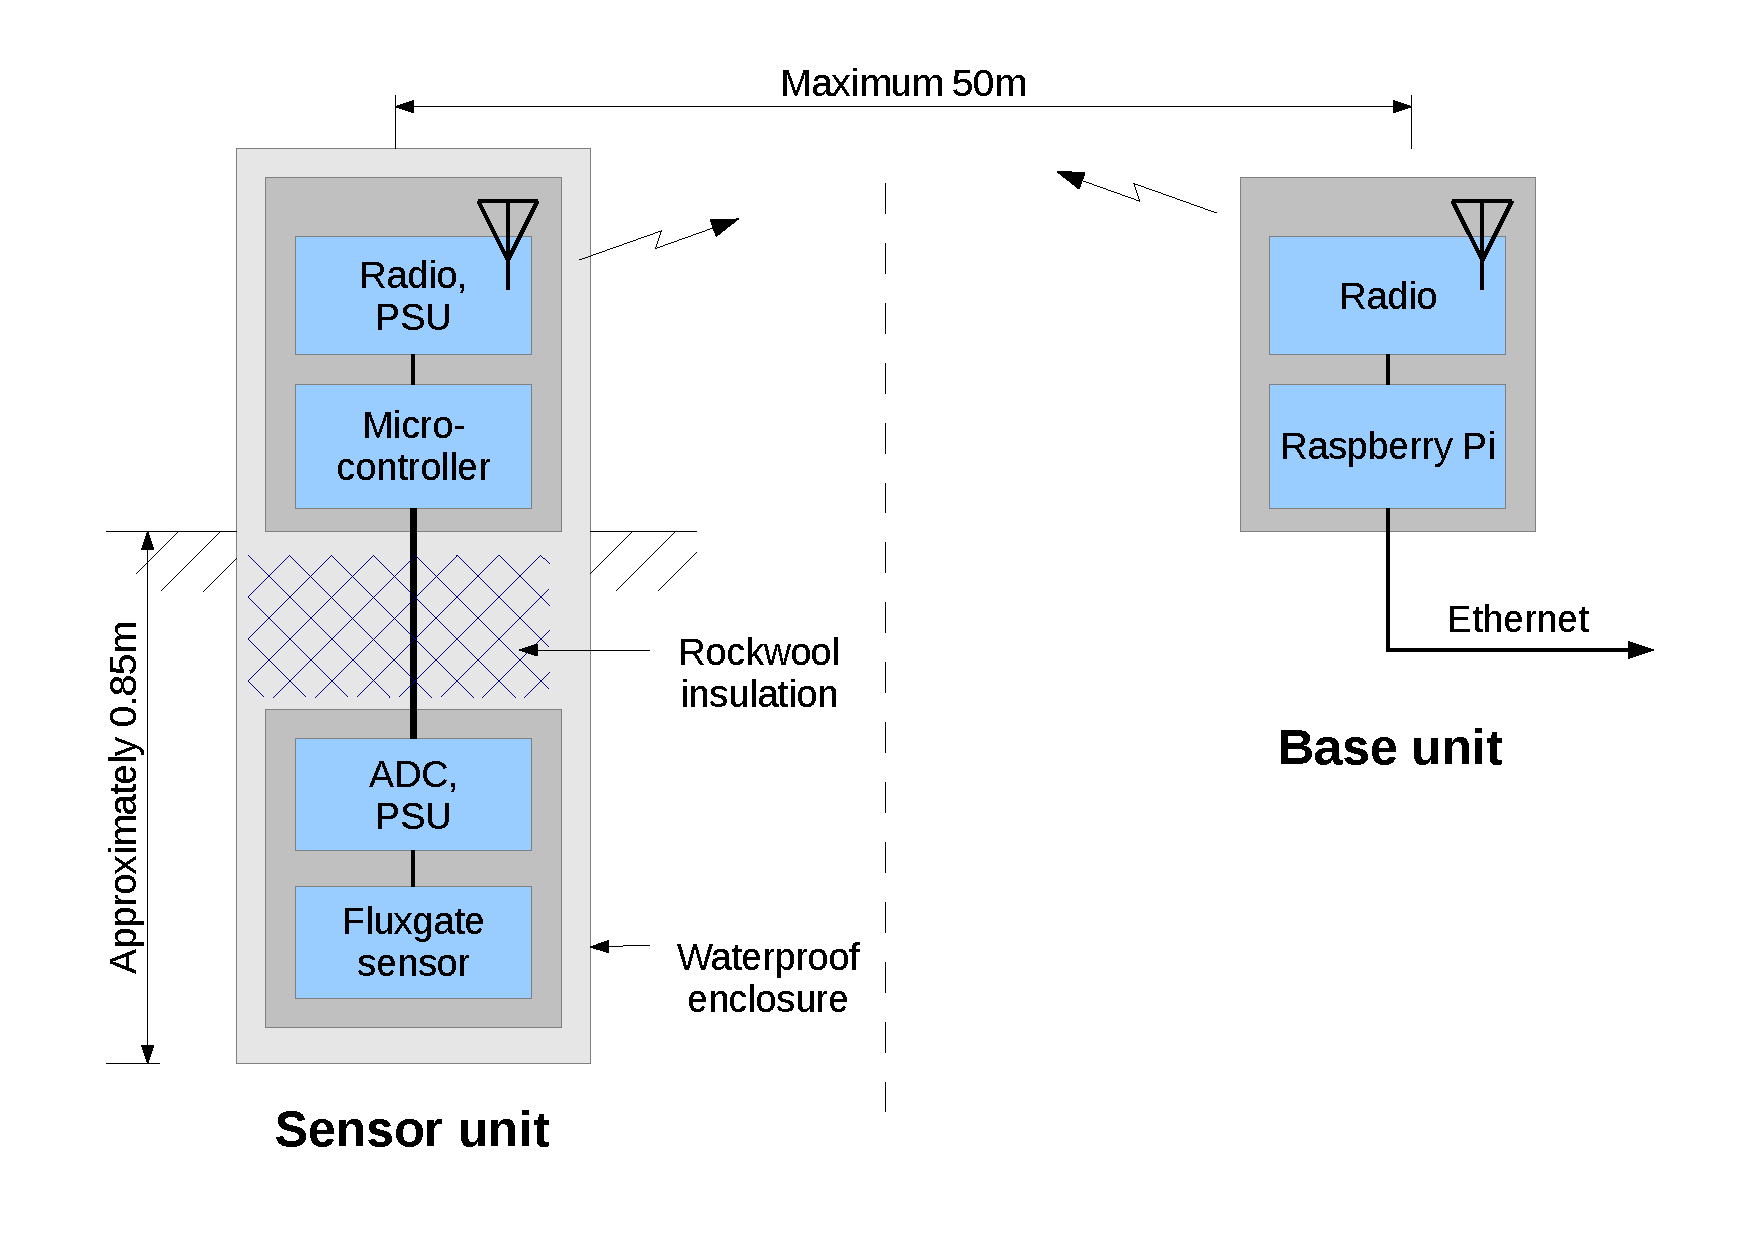
\includegraphics[keepaspectratio,width=\textwidth]{images/system-overview}
  \caption[System overview]%
  {System overview.}
  \label{fig:system-overview}
\end{figure}

\section{Sensor unit}

\begin{figure}
  \centering
  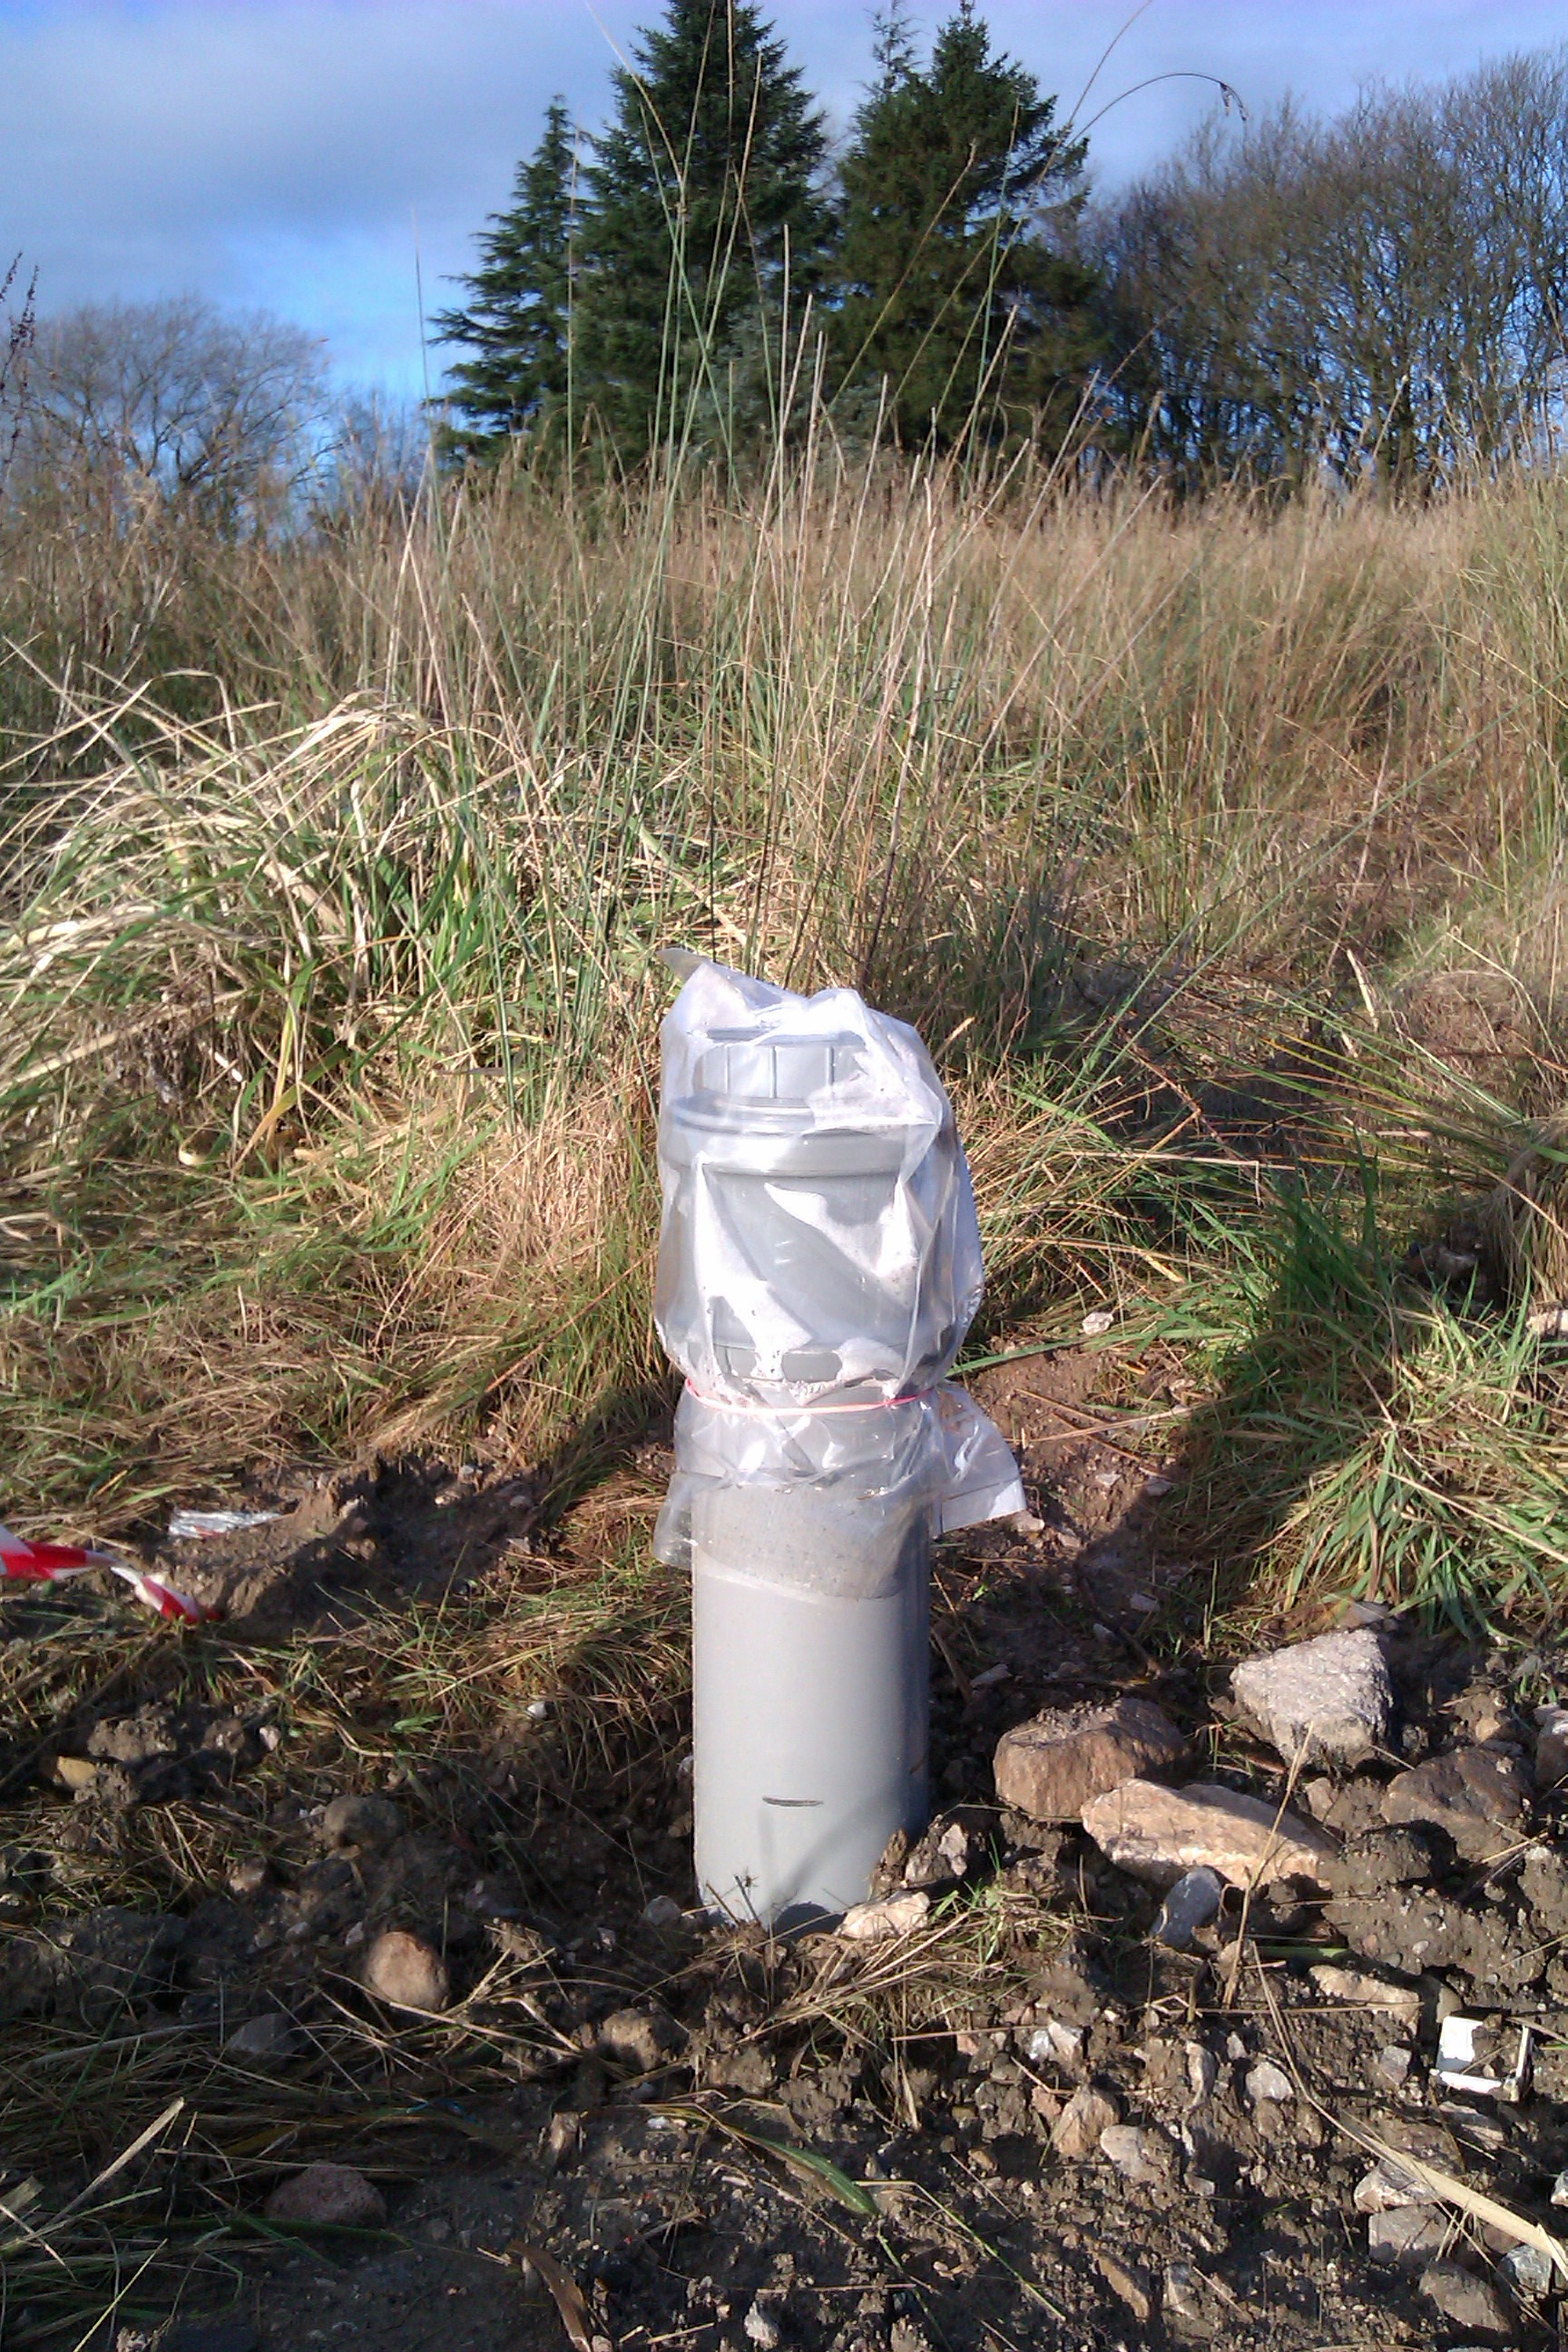
\includegraphics[keepaspectratio,height=10cm]{images/sensor-unit}
  \caption[Sensor unit]{%
    Sensor unit. \photoCredits{%
      \href{http://www.flickr.com/photos/stevemarple/8499204572/}{%
        \copyright Steve Marple. CC BY-SA 3.0.}}}
  \label{fig:sensor-unit}
\end{figure}

The sensor unit is contained inside a waterproof enclosure
approximately \SI{1.1}{\metre} high which is partially buried to reduce
temperature variations and to provide a stable foundation. The sensor
itself is placed at the bottom of the enclosure, approximately
\SI{0.85}{\metre} below ground. The microcontroller, radio module and
battery are positioned in the top part of the enclosure, above ground
level. Insulating material (\eg\ rockwool) is used to fill the space
in-between.

The
\href{http://blog.stevemarple.co.uk/search/label/Calunium}{Calunium}
microcontroller board is based on the popular
\href{http://arduino.cc}{Arduino} platform but uses the more powerful
Atmel ATmega1284P microcontroller.

\section{Base unit}

\begin{figure}
  \centering
  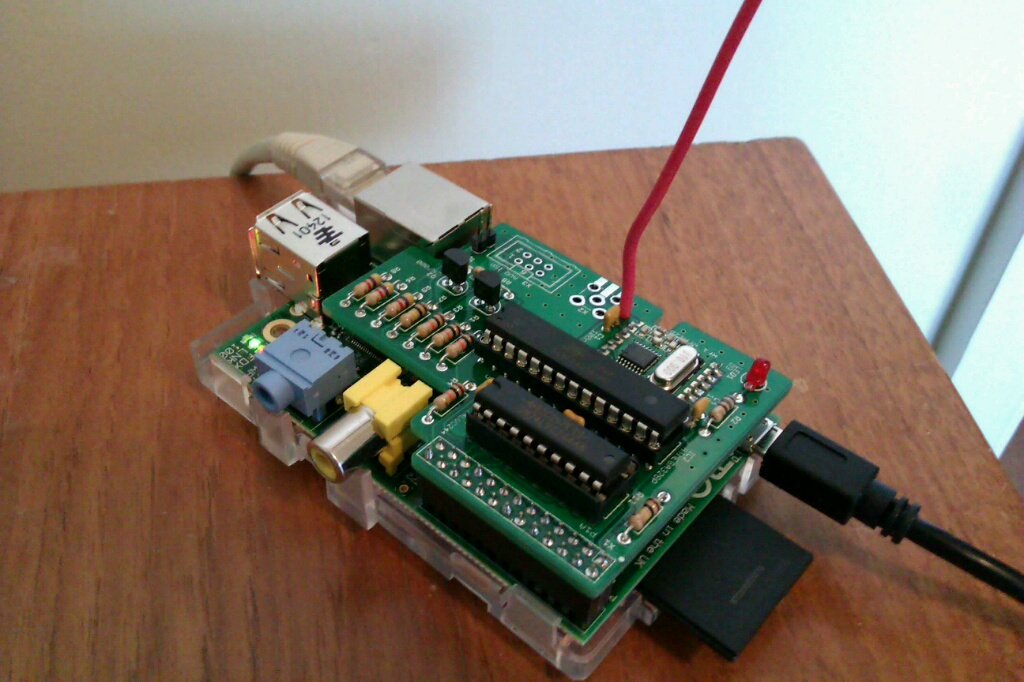
\includegraphics[keepaspectratio,height=10cm]{images/base-unit}
  \caption[Base unit]{%
    Base unit. \photoCredits{%
      \href{http://www.flickr.com/photos/stevemarple/10787215844/}{%
        \copyright Steve Marple. CC BY-SA 3.0.}}}
  \label{fig:base-unit}
\end{figure}

The base unit is a \href{http://www.raspberrypi.org/‎}{Raspberry Pi}
single-board computer with a radio transceiver unit. The Ethernet
interface of the Raspberry Pi is used to send the magnetic field
measurements to AuroraWatch UK. When the Raspberry Pi is accessed over
the network with Secure Shell (\ssh) a display and keyboard are not
needed. The Raspberry Pi runs the Raspbian linux distribution. The
receiving software is written in Python.

